\chapter{Methodik}
In diesem Kapitel wird die methodische Vorgehensweise der Arbeit präsentiert. Zunächst wird die Einrichtung der Hardware beschrieben, einschließlich Details zu Art und Konfiguration der verwendeten Hardwarekomponenten. Diese Erläuterung bietet den Lesern einen umfassenden Überblick über den Laboraufbau und fungiert als Referenzpunkt für etwaige Nachahmungsstudien. Als nächstes erfolgt die Darstellung des Trainingsprozesses des YOLO-Detectors, einschließlich der verwendeten Daten und Markierungsmethoden. Hierdurch wird ein detailliertes Verständnis für die angewandte Methodik zur Objekterkennung vermittelt. Abschließend wird die Implementierung der Bot-SORT als Tracker präsentiert. Durch geringfügige Modifikationen im Algorithmus wurde eine signifikante Reduzierung von ID-Switch erreicht, was auf eine verbesserte Verfolgungsgenauigkeit hinweist.

\section{Hardware-Einrichtungen}   
    Die in dieser Arbeit verwendete Zugprüfmaschine ist horizontal positioniert \ref{fig:methodik:myZugprüfmaschine}. Sowohl der dynamische als auch der statische Traverser verfügen über eine runde Palette, die in der Lage ist, gleichzeitig 8 Testproben zu fixieren. Die Elastomerproben werden in flacher Sanduhr-Form gestaltet. Ein Testlauf mit 8 Testproben gleichzeitig ist produktiver und wirtschaftlicher als herkömmliche Zugversuche mit nur einer Probe. Dies ermöglicht es, in einem einzigen Testlauf mit einer definierten Spannung gleichzeitig 8 verschiedene Materialien zu prüfen und den Prüfprozess dadurch zu beschleunigen. Ein Nachteil besteht jedoch darin, dass die hinteren Proben erheblich von den vorderen Proben überlappt werden. Dieses Problem beeinträchtigt die Fähigkeit des Detektors, die überlappenden Proben zu erkennen, und führt daher zu einer verringerten Leistung des Detektors. Umgebung und Traverser sind durch eine Box begrenzt, sodass eine Temperaturbeeinflussung möglich ist. Bei Temperaturbeeinflussung wird die Box mit einer Decke abgedeckt und bis zu einer definierten Temperatur erhitzt. Beim Temperaturtest gibt es ein Problem: Die Testproben werden von der Decke abgedeckt und können nicht von der Kamera oben beobachtet werden. Aus diesem Grund konzentriert sich diese Arbeit auf die Erkennung von gerissenen Proben bei Raumtemperatur.

    \begin{figure}[htbp]
        \centering
            \subfigure[]{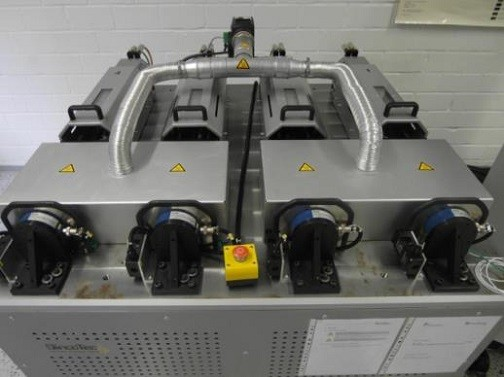
\includegraphics[width=0.49\textwidth, height=0.33\textwidth]{gfx/Hardware/TestMaschine_1.png}}
            \subfigure[]{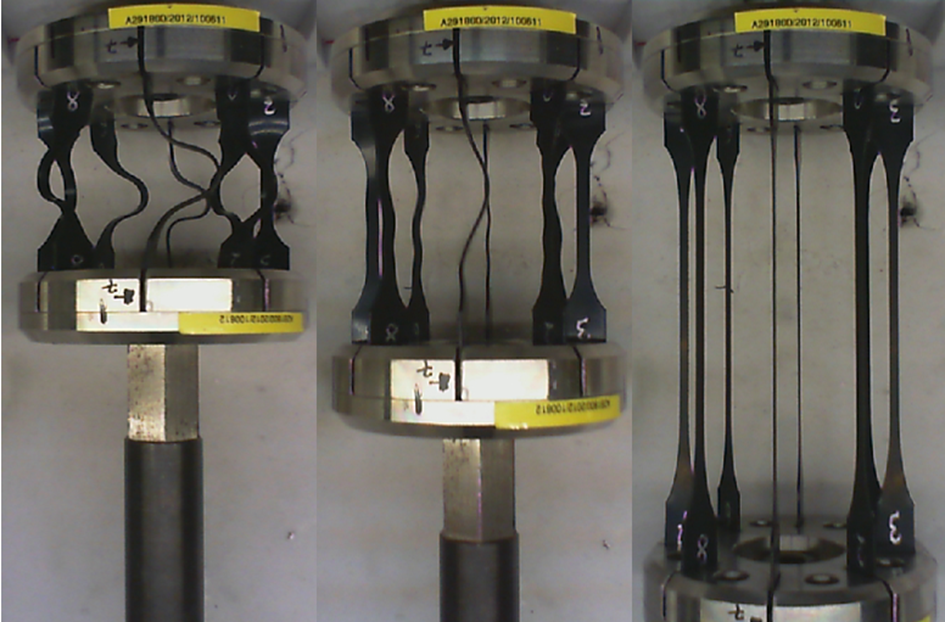
\includegraphics[width=0.5\textwidth]{gfx/Hardware/TestMaschine_2.png}}
            \caption[Die verwendete Zugprüfmaschine.]{(a): Die Zugprüfmaschine zum Ermüdungstest unter Temperatureinfluss. Quelle: \cite{zyklischePrüfung}. (b) Draufsichten auf das Prüfgerät mit 8 Elastomerproben. Eine Traverser ist feststehend, die andere wird horizontal zyklisch bewegt. Quelle: Eigene Quelle. (c) Fotos von Testproben mit nahem View.}
            \label{fig:methodik:myZugprüfmaschine}
    \end{figure}

    Während des Testdurchlaufs wird das Video des Testlaufs mithilfe eines Raspberry Pi 5 über das Netzwerk zum Server gestreamt. Auf dem Server läuft gleichzeitig die KI-System, um die gerissenen Proben in Echtzeit zu erkennen. Der Server verfügt über eine NVIDIA A30 Grafikkarte \cite{graphiccard} und eine Intel(R) Xeon(R) Gold 6250 3.90GHz CPU \cite{cpu}. Die verwendete Kamera ist die RASP CAM HQ \cite{camera} mit einem 16mm Teleobjektiv RPIZ CAM 16MM TO \cite{camera}. 

    Für jede Achse der Zugprüfmaschine wird eine Kamera präzise mit einem festgelegten Abstand und Winkel positioniert. Die genaue Anordnung und der Winkel zwischen der Kamera und den Testproben spielen eine entscheidende Rolle für die Effektivität des Detektors. Die Kamera und die Testproben müssen so positioniert werden, dass Überlappungen so weit wie möglich minimiert werden. Vollständige Vermeidung von Überlappungen ist jedoch nicht in jedem Fall möglich, da die Testproben um die Achse fixiert sind. In Abbildung \ref{fig:methodik:falsePosition} werden schlechte Positionen der Testproben veranschaulicht, die durch gelbe Ellipsen gekennzeichnet sind. In diesen Positionen kommt es zu erheblichen Überlappungen, wobei die hintere Probe sich deutlich (fast zu 100\%) mit der vorderen Probe überschneidet.

    \begin{figure}[htbp]
        \centering
            \subfigure{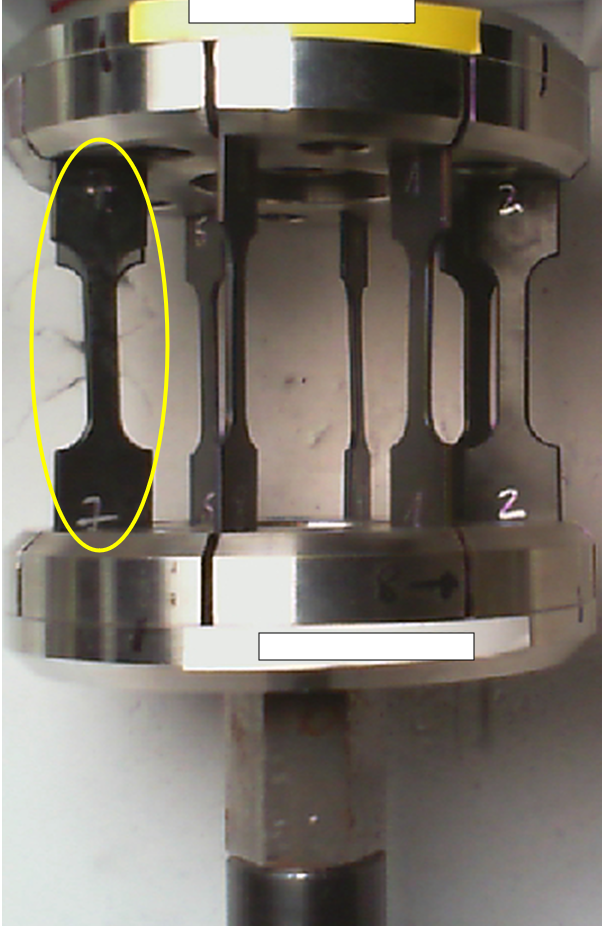
\includegraphics[width=0.24\textwidth, height=0.34\textwidth]{gfx/Hardware/BadPos_1.png}}
            \subfigure{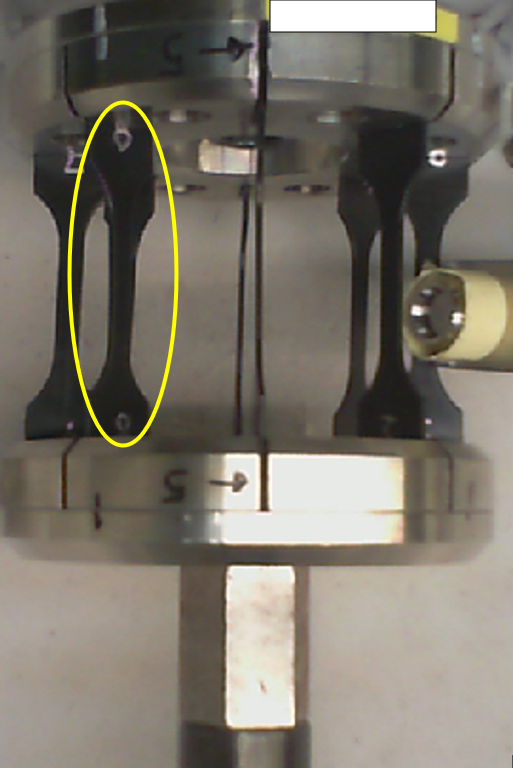
\includegraphics[width=0.24\textwidth, height=0.34\textwidth]{gfx/Hardware/BadPos_2.png}}
            \subfigure{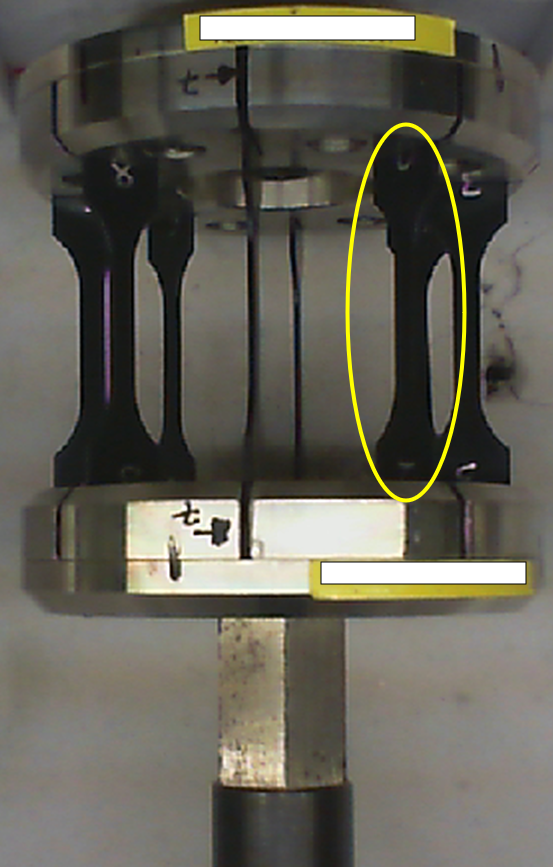
\includegraphics[width=0.24\textwidth, height=0.34\textwidth]{gfx/Hardware/BadPos_3.png}}
            \subfigure{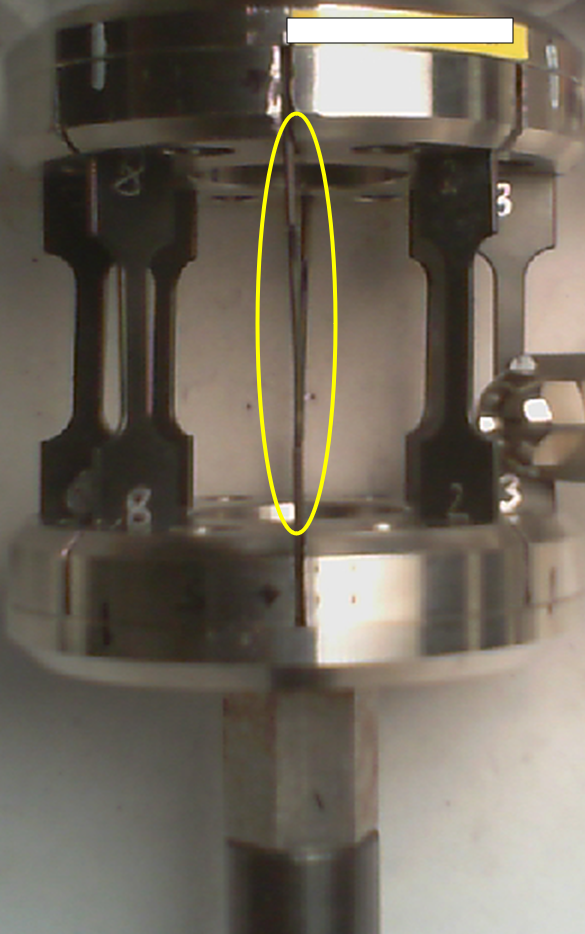
\includegraphics[width=0.24\textwidth, height=0.34\textwidth]{gfx/Hardware/BadPos_4.png}}
            
            \caption[Schlechte Positionen der Testproben.]{Die gelben Ellipsen markieren die schlechten Positionen, in denen es zu erheblichen Überlappungen kommt.}
            \label{fig:methodik:falsePosition}
    \end{figure}

    In Abbildung \ref{fig:methodik:rightPosition} sind alle Testproben in optimalen Positionen dargestellt, wobei die Überlappungen, die durch rote Ellipsen markiert sind, auf ein Minimum reduziert werden. Trotzdem bleibt ein großer Anteil der überlappenden Proben deutlich sichtbar. In einer optimalen Konfiguration sollten 70\% der überlappenden Testproben sichtbar sein. Die Ausrichtung der Kamera erfolgt heuristisch, um sicherzustellen, dass sich alle Testproben in optimalen Positionen befinden. Eine umfassende, systematische Methode zur Bestimmung der Kameraposition liegt jedoch außerhalb des Umfangs dieser Arbeit.
    
    \begin{figure}[htbp]
        \centering
            \subfigure{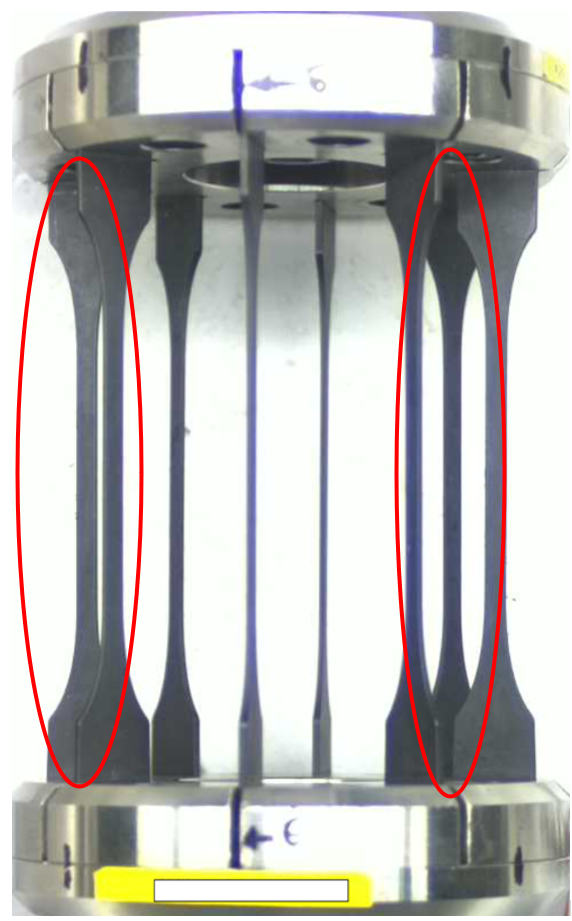
\includegraphics[width=0.24\textwidth, height=0.34\textwidth]{gfx/Hardware/GoodPos_1.png}}
            \subfigure{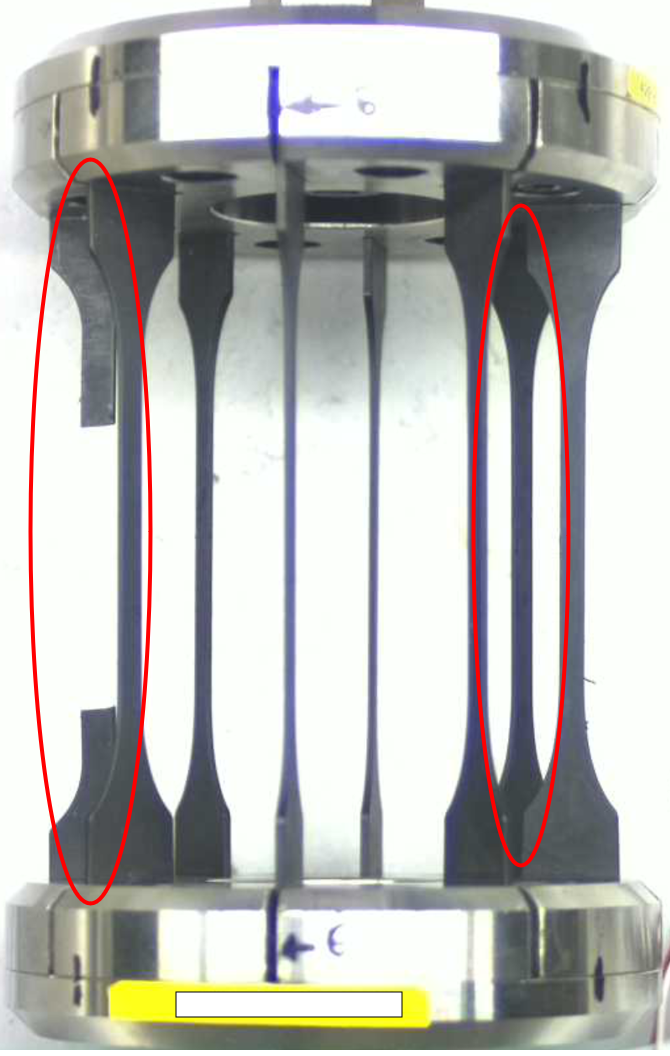
\includegraphics[width=0.24\textwidth, height=0.34\textwidth]{gfx/Hardware/GoodPos_2.png}}
            \subfigure{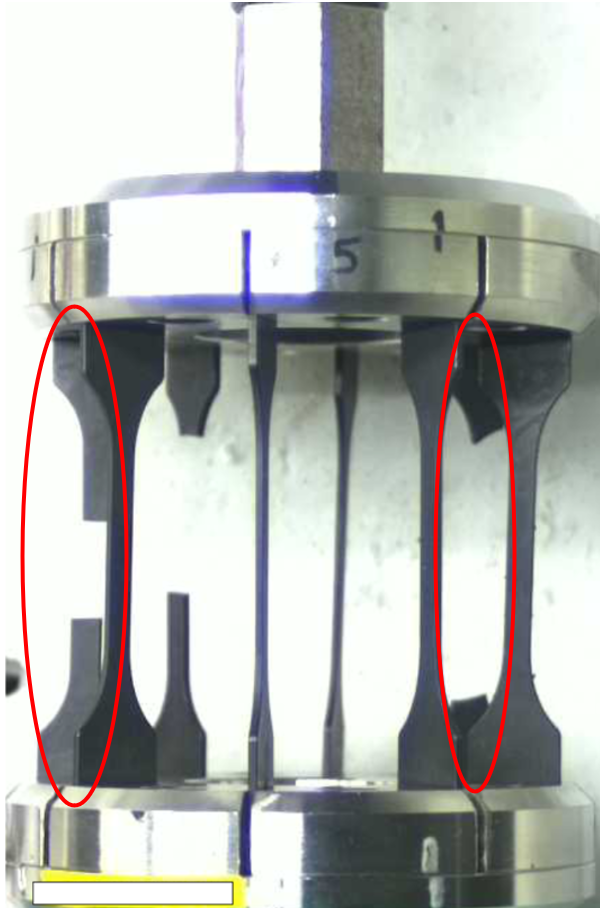
\includegraphics[width=0.24\textwidth, height=0.34\textwidth]{gfx/Hardware/GoodPos_3.png}}
            
            \caption[Gute Positionen der Testproben.]{Eine gute Konfiguration der Testproben verdeutlicht, dass ein großer Anteil der überlappenden Proben (gekennzeichnet durch rote Ellipsen) klar erkennbar ist.}
            \label{fig:methodik:rightPosition}
    \end{figure}

    \textbf{(Ein Absatz über Brightless und Contrast)}
\section{Detector}
Wie im ersten Kapitel bereits besprochen, wird YOLO als der eingesetzte Detektor verwendet. In diesem Unterkapitel wird die Implementierung des Detektors näher erläutert. Zunächst erfolgt eine Vorstellung des Labelings von Objekten, gefolgt von einer Erläuterung der Datensätze für das Training von YOLO. Abschließend werden das Training und die erzielten Ergebnisse behandelt.

    \subsection{Labelling} 
    Labelling ist ein bedeutender Prozess, der einen entscheidenden Einfluss auf die Performance des Detectors ausübt. In dieser Arbeit wurden drei unterschiedliche Labelling-Methoden ausprobiert, und die Performance des Modells wird für jede dieser Methoden bewertet. In allen Methoden werden ausschließlich Testproben berücksichtigt, bei denen ein Riss auftritt. Dies geschieht, da die Überlebenszeit nur für diese Testproben erfasst werden soll. 

    In der ersten Methode \ref{fig:methodik:Labelling-Methods} (a) wird ausschließlich die Klasse "broken" verwendet, um die gesamte gerissene Probe, sowohl den oberen als auch den unteren Teil, innerhalb einer Bounding Box zu markieren. In der zweiten Methode \ref{fig:methodik:Labelling-Methods} (b) hingegen erfolgt eine differenzierte Klassifizierung der gerissenen Teile in die Kategorien "top" und "bottom". Diese präzise Positionsinformation innerhalb der Klassen gewinnt besondere Bedeutung für die Anpassung des BotSort-Algorithmus im darauf folgenden Kapitel. Die dritte Methode \ref{fig:methodik:Labelling-Methods} (c) gleicht der zweiten Methode in Bezug auf die Klassifizierung von "top" und "bottom", fügt jedoch eine zusätzliche Klasse namens "Box" für die Probenaufnahme hinzu.

    \begin{figure}[htbp]
        \centering
        \subfigure[]{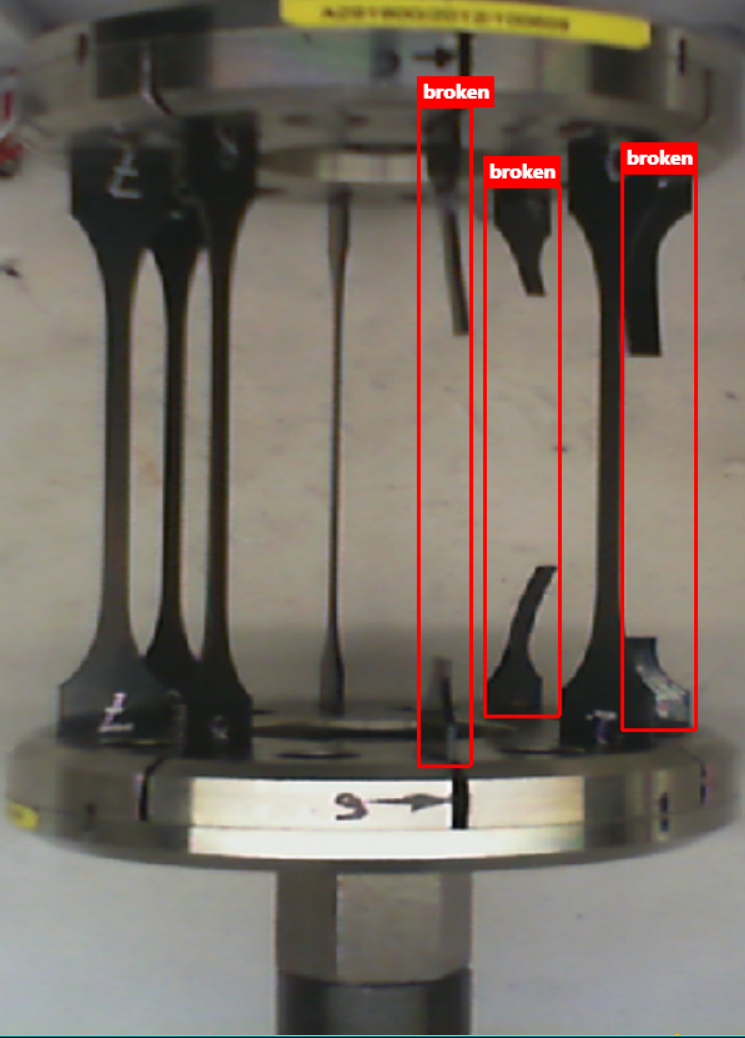
\includegraphics[width=0.32\textwidth, height=0.45\textwidth]{gfx/Detector/Labeling/Methode_1.png}}
        \subfigure[]{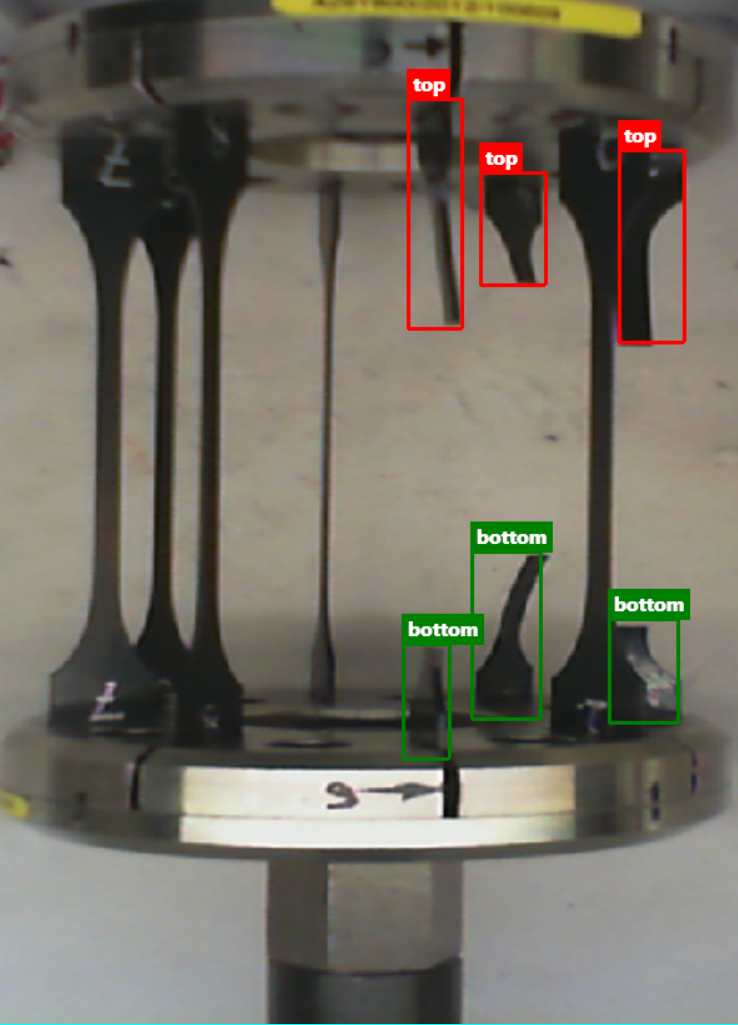
\includegraphics[width=0.32\textwidth, height=0.45\textwidth]{gfx/Detector/Labeling/Methode_2.png}} 
        \subfigure[]{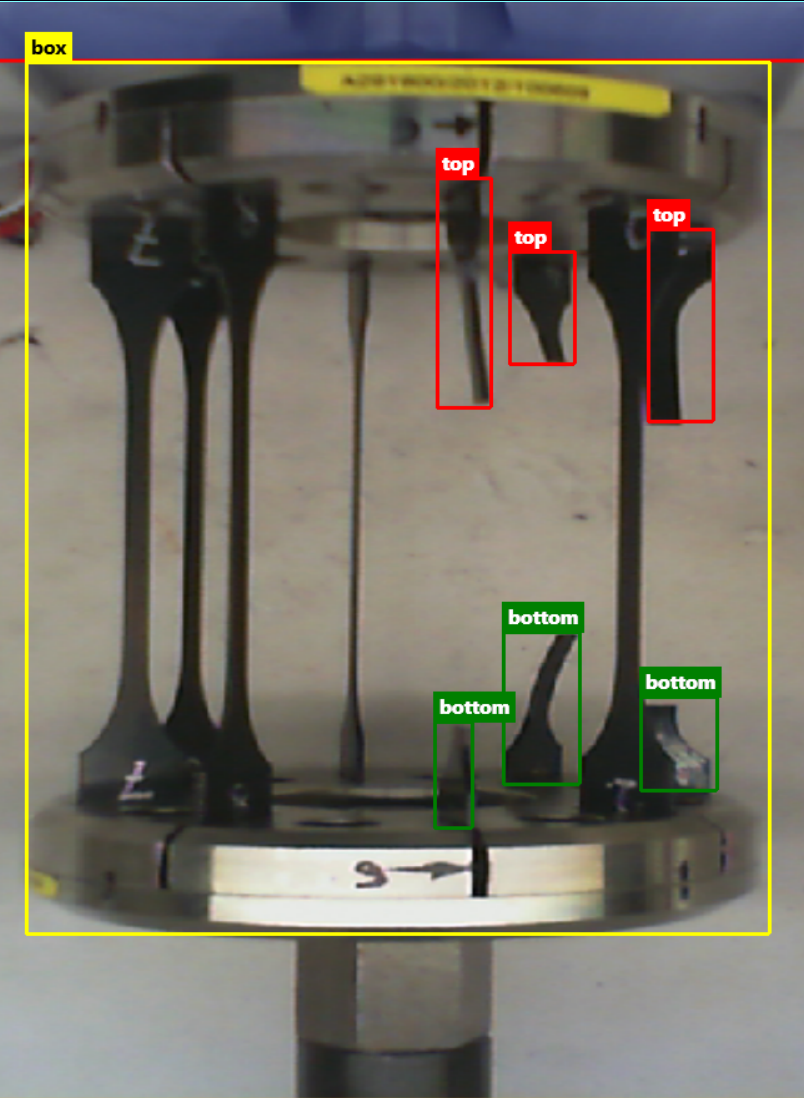
\includegraphics[width=0.32\textwidth, height=0.45\textwidth]{gfx/Detector/Labeling/Methode_3.png}}
    
        \caption[Drei Labeling-Methoden.]{(a) Methode 1. (b) Methode 2. (c) Methode 3.}
        \label{fig:methodik:Labelling-Methods}
    \end{figure}

    In Abbildung \ref{fig:methodik:Labelling-Performance} wird die Performance von Yolov8 Nano anhand identischer Trainingsdaten unter Verwendung von drei verschiedenen Labelling-Methoden dargestellt. Die Trainingsdaten und Testdaten, die für den Vergleich verwendet wurden, werden im nächsten Abschnitt erläutert. Die erste Methode weist die schwächste Performance auf (58.1\% mAP@50-95), gefolgt von der zweiten (75.5\%) und der dritten Methode (82.8\%). Die Ursache für die geringe Performance der ersten Methode könnte darin liegen, dass die Bounding Box viele Störungen enthält, sprich die Pixel zwischen dem oberen und unteren Teil der gerissenen Probe. Im Gegensatz dazu erzielt die dritte Methode eine bessere Performance als die zweite, obwohl sie nur eine zusätzliche Klasse ("Box") im Vergleich zur zweiten Methode aufweist.

    \begin{figure}[htbp]
        \centering
        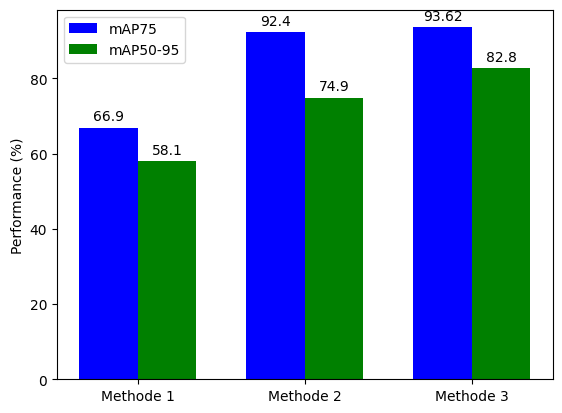
\includegraphics[width=0.65\textwidth]{gfx/Detector/Labeling/Labeling_Performance.png}
        \caption[Performancevergleich zwischen drei Labeling-Methoden.]{Performancevergleich zwischen drei Labeling-Methoden unter Verwendung von YOLOv8 Nano anhand mAP75 und mAP50-95.}
        \label{fig:methodik:Labelling-Performance}
    \end{figure}

    Die Tabelle \ref{tab:Labelling_Performance} zeigt, dass die Klasse "Box" der Methode 3 von Yolov8 nahezu fehlerfrei erkannt wird (fast 100 \% mAP50-95). Diese präzise Erkennung der Probenaufnahme trägt dazu bei, die Gesamtperformance zu steigern, während die Performances der beiden anderen Klassen fast unverändert bleiben. Dies ist verständlich, da die Probenaufnahme ziemlich konstant bleibt und keine Überlappungen aufweist. Eine hohe Konfidenz bei der Erkennung der Probenaufnahme ist von entscheidender Bedeutung, da sie als Grundlage für zukünftige Funktionen dient, die im nächsten Kapitel besprochen werden (die Vermeidung von Überlappungen und die Zählung von Zyklen). Aus diesen Gründen wurde die dritte Labelling-Methode für die Daten  verwendet.

    \begin{table}[htbp]
        \myfloatalign
        \begin{tabular}{ccccc} 
                \tableheadline{} & 
                \tableheadline{Top} & 
                \tableheadline{Bottom} &
                \tableheadline{Box} &
                \tableheadline{Gesamt}\\ 
            \midrule
                Methode 2 & 75\% & 74.8\% & None & 74.9\% \\
                Methode 3  & 74.6\%  & 74.4\%  & 99.5 \% & 82.8\%
        \end{tabular}
        \caption[Klassperformance in Methode 2 und 3.]{Die Performance der Methoden 2 und 3 wurde für jede Klasse anhand mAP50-95 bewertet. Da Methode 2 keine Klasse ''Box'' aufweist, wurde dieser Wert als 'None' angegeben. Die Gesamtperformance wurde als Durchschnitt berechnet.}
        \label{tab:Labelling_Performance}
    \end{table}

    \subsection{Datensätze}
    Der Trainingsdatensatz besteht aus 5330 Bildern, die während 81 Testdurchläufen aufgenommen wurden. Im Testdatensatz sind 676 Bilder aus 7 Testdurchläufen enthalten. Um den Trainingsdatensatz zu generieren, wurde jedes Bild während eines Testdurchlaufs alle 60 Sekunden aufgenommen, was zu durchschnittlich 6000 Bildern pro Testdurchlauf führte. Eine charakteristische Eigenschaft von Ermüdungstests ist die repetitive Bewegung der dynamischen Traverse und der Testproben in jedem Zyklus, was zu sehr ähnlichen Daten in den 6000 Bildern führt. Da eine große Menge identischer Bilder die Leistung des Modells nicht verbessert, sondern nur den Trainingsprozess verlangsamt und einen voreingenommenen Datensatz bildet, werden nur Bilder aus zwei Zyklen gesammelt, nachdem eine Testprobe gerissen ist. Durch dieses Filtern von identischen Bildern wird die Anzahl der Trainingsdaten von 486,000 Bildern auf 5330 Bilder reduziert, ohne dabei die Varianz der Daten zu beeinträchtigen. Das bedeutet, dass von den ursprünglichen 6000 Bildern pro Testdurchlauf nun nur etwa 65 Bilder verwendet werden.

    \begin{table}[htbp]
        \myfloatalign
        \begin{tabular}{lccc} 
                \tableheadline{} & 
                \tableheadline{Gesamt} & 
                \tableheadline{Hintergrundbilder} &
                \tableheadline{Durchläufe}\\ 
            \midrule
                Training & 5330 & 747 (14\%) & 81 \\
                Test  & 676 & 67 (9.9 \%) & 7 
        \end{tabular}
        \caption[Datensätze.]{Information über die Datensätze.}
        \label{tab:Datasets}
    \end{table}

    Hintergrundbilder oder  ...

    Abbildung \ref{fig:methodik:Datensatz} zeigt die Verteilung der Klassen im Trainings- und Testdatensatz nahezu identisch, was auf die Eigenschaft des Ermüdungstests zurückzuführen ist. Die Anzahl der Instanzen von ''Box'' beträgt immer 1 pro Bild, während die Anzahl von ''Top'' und ''Bottom'' beim Riss einer Testprobe gleich ist, es sei denn, sie überlappen sich. Diese Charakteristik führt zu einer geringen Varianz in den Anteilen der Klassen zwischen Trainings- und Testset. Das bedeutet, dass das Testset die Klassenverteilung des Trainingsets sehr gut repräsentiert. Die Anzahl der Instanzen für jede Klasse im Trainingsdatensatz liegt bei etwa 18.000 für ''Top'' und ''Bottom'', was für diese Aufgabe mit konstantem Hintergrund und geringer Varianz in der Objektform ausreicht. Im Vergleich dazu haben beliebte Datensätze wie COCO \cite{COCO} durchschnittlich 10.000 Instanzen pro Klasse und PASCAL VOC 2012 \cite{PASCAL} zwischen 500 und 10.000 Instanzen pro Klasse. Eine Ausnahme bildet die Klasse ''Box'' mit nur 5.000 Instanzen. Dies stellt jedoch kein Problem dar, da diese Klasse sehr gut sichtbar ist (ohne Überlappung) und sich nur minimal bewegt.

    \textbf{Explain why down split the dataset to 80-20.}
    
    \begin{figure}[htbp]
        \centering
        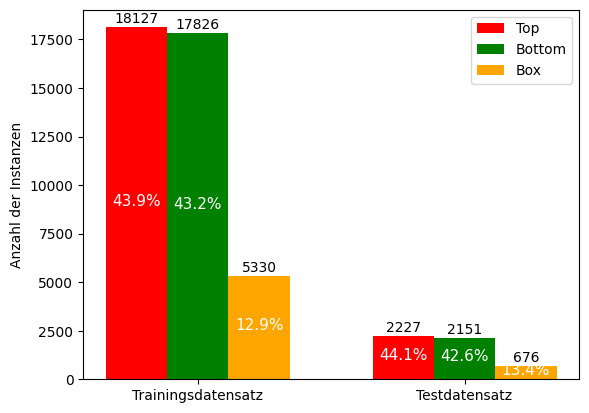
\includegraphics[width=0.7\linewidth, height=0.5\textwidth]{gfx/Detector/Dataset/Datensatz.png}

        \caption[Die Verteilung der Klassen in Trainings- und Testdatensatz]{Die Klassenverteilung im Trainings- und Testdatensatz. Der Anteil jeder Klasse wird in der Mitte jeder Klassebar angezeigt.}
        \label{fig:methodik:Datensatz}
    \end{figure}

    Ein weiterer außer wichtiger Punkt, der den Modell's Performance erheblich beeinflussen kann, ist die Varianz der Trainingsdaten. die Trainingsdaten soll alle mögliche Szenarien in Realität repräsentieren, wie Beleuchtung, Objektsgröße, Hintergrund (kann in diesem Problem beeinträchtigt), Defektform, etc. Eine hohe Varianz der Trainingsdaten verhindert, dass der Modell das Bias lernt und gute Performance beim Testen aber schlechte Performance in der Realität ergibt. Dafür wurden die Trainingsdaten aus 81 Testdurchläufe in dieser Arbeit mit möglichst vielen unterschiedlichen Kameraswinkels, Abstände zwischen die Testproben und den Kamera, Defektformen der Testproben generiert. Defektformen unterscheiden sich abhängig vom Probenmaterial, Risspunkt, Testfrequenz und Amplitude. In Trainingsdaten können alle Defekten hauptsächlich in 4 verschiedenen Defektformen. Die erste Form hat eine mittlere Größe und kann vom YOLO wegen klares Aussehens und seiner Größe am besten erkannt werden. Diese Defektform entsteht normalerweise bei Proben mit hartem Material und in einem Testlauf mit kleinerer Amplitude. Die zweite Defektform ist von den Proben an der Mitte, die eine schmale Form haben. Diese Defektform kann auch sehr gut erkannt werden, weil sie unter keine Überlappung leiden. Bei der vierte Defektform wird die Probe sehr viel verformt und verlängert. Diese Defektform  hat die größte Größe und entsteht bei weichen Materialen und Tests mit großer Amplitude. Die letzte Defektform passiert, wenn der Risspunkt entweder an obere oder untere Ende einer Probe liegt, was dazu führt, dass eine   

    \subsection{Performance Metrik}
    
    
    \subsection{Training}
    \subsection{Ergebnisse}
\section{Tracker}
